\section{The Symmetry Breaking Problem}
\label{cap:2}

Formally, a symmetry system can be defined as a system in which the processes are in an equivalence relation, this means that if the processes run the same code, it is possible to permute the nodes without changing the behaviour of the system. One example of this state would be a ring in which there is no unique identifier for every node. If we consider a message passing system in which the initial state of symmetry between all processes, it is possible to find a synchronous execution in which the processes will continue in the same initial state. In this case, it is necessary a mechanism to break the symmetry, in the contrary, the system cannot escape from the initial state.
%as shown in \cite{angluin1980local} by Angluin.

Symmetry breaking is one of the most extensively studied problems in distributed computing. The fundamental problems on graph include the maximal matching, vertex colouring, ruling sets and \textit{MIS}. The last one can be considered as the central problem because all the others can be reduced to it, as shown in  \cite{}.

Next, in this chapter a formal definition of the maximal independent set is given and two algorithms are presented to solve the problem. Besides that, a theoretical analysis about the time and message complexity is described.     

\subsection{Maximal Independent Set}

\theoremstyle{definition}
\begin{definition}

Given a undirected graph $G = (V,E)$, a set of vertices $S \subseteq V$ is called a Maximal Independent Set \textbf{MIS} if it satisfied the following properties:   

\begin{enumerate}
  \item the set S in an independent set meaning that no two vertices $v,u \in S$ are adjacent,
  \item the set S is maximal, with regards to independence, meaning that for each node $v \notin S$, there 
    exist a neighbour u of v such that $u \in S$.
\end{enumerate}

\end{definition}

Figure \ref{fig:graph1} show an example of undirected graph with 8 nodes and 14 edges. The goal if to find a set of nodes in which every node is part of the set or it is neighbour of some node that is part of the set. It is possible to find more that one solution to the same instance as shown in the figure \ref{fig:mis1}  
 
\begin{figure}[h]
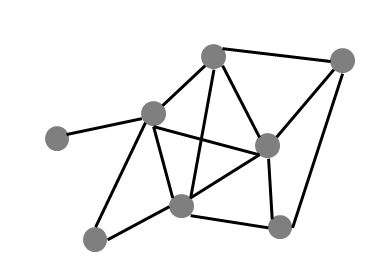
\includegraphics[width=0.4 \linewidth, height=3cm]{c2-graph.PNG} 
\caption{General graph G}
\label{fig:graph1}
\end{figure}
 
\begin{figure}[h]
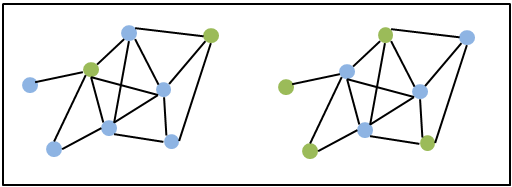
\includegraphics[width=0.4 \linewidth, height=3cm]{c2-graph-mis1.PNG}
\caption{Solution 1 for MIS of G}
\label{fig:mis1}
\end{figure}

The algorithm \ref{algorithm:secuential-mis} describe a general sequential algorithm to find the maximal independent set of a general graph. The time complexity is $O(N)$. Since in the worst case, the sequential algorithm has to check every node, another approach that improve this time is desirable. In the next section, the distributed approach to solve the \textit{MIS} problem is presented.

\begin{algorithm}
 \caption{Sequential Maximal Independent Set}
 \label{algorithm:secuential-mis} 

\SetAlgoLined
\KwResult{IS Set of nodes}
\KwData{ $G(V,E)$ Graph}
    \While {V is not empty}{
        Choose a node $v \in V$
            Add v to the set IS\;
            Remove from V the node v and all its neighbours\;
        }
    
 
\end{algorithm}
 

 
\subsection{Distributed Maximal Independent Set}
fsdfsdfsdfsdfsd
\newpage

